\documentclass{book}
\usepackage[utf8]{inputenc}
\usepackage{amsmath}
\usepackage{amsfonts}
\usepackage{esint}
\usepackage{geometry}
\usepackage{color}
\usepackage{fancyhdr}
\usepackage{ctable}
\usepackage{fancybox}
\usepackage{tabularx}
\usepackage{array}
\usepackage{booktabs}
\usepackage[french]{babel}
\usepackage{dsfont}
\usepackage{setspace}
\usepackage[french]{minitoc}
\usepackage{multicol}
\usepackage{multirow}
\usepackage[hidelinks]{hyperref}
\usepackage{graphicx}
\usepackage[T1]{fontenc}
\usepackage{xcolor}
\usepackage{listings}

\geometry{top=2.5cm, bottom=2.5cm, left=3cm, right=3cm}

\addtocounter{tocdepth}{3}
\setcounter{secnumdepth}{3}


\definecolor{codegreen}{rgb}{0,0.6,0}
\definecolor{codegray}{rgb}{0.5,0.5,0.5}
\definecolor{codepurple}{rgb}{0.58,0,0.82}
\definecolor{backcolour}{rgb}{0.95,0.95,0.92}

\lstdefinestyle{mystyle}{
  backgroundcolor=\color{white}, commentstyle=\color{codegreen},
  keywordstyle=\color{magenta},
  numberstyle=\tiny\color{codegray},
  stringstyle=\color{codepurple},
  basicstyle=\ttfamily\footnotesize,
  breakatwhitespace=false,         
  breaklines=true,                 
  captionpos=b,                    
  keepspaces=true,                 
  numbers=left,                    
  numbersep=5pt,                  
  showspaces=false,                
  showstringspaces=false,
  showtabs=false,                  
  tabsize=2
}

\lstset{style=mystyle}

\begin{document}

%%%%%%%%%%%%%%%%%%%%%%%%%%%%%%%%%%%%%%%%%%%%%%%%%%%%%%
%%%%%%%%%%%%%%%%%%%% PRÉSENTATION %%%%%%%%%%%%%%%%%%%%
%%%%%%%%%%%%%%%%%%%%%%%%%%%%%%%%%%%%%%%%%%%%%%%%%%%%%%

\begin{titlepage}

    \unitlength 1cm
    \begin{center}
    
    \vspace*{1cm}

    
\includegraphics[scale=0.6]{figures/logo_ico.png}
    
    \vspace{2cm}
    
               {\Large Diplôme de Qualification en Physique Radiologique et Médicale\\}
               
    \vspace{2cm}           
    
    
    \rule{16cm}{0.7pt}
    
    \vspace{12pt}
               
               {\LARGE \bf Faisceaux de photons de haute énergie : cas des petits faisceaux\\}
               
    \vspace{12pt}
    \rule{16cm}{0.7pt}

    \vspace{2cm}

                {\large Fiche n°3b}
    
    \vspace{1.5cm}

               {\Large\bf {Alexandre \textsc{Rintaud}}}
    
    \vspace{1.5cm}
    
    \end{center}
    
    Encadrants :
    
    \small {
    \begin{tabular}{llr}\\
    \textbf{Stéphanie \textsc{Josset}}   &  &  \\
      Physicienne médicale, \textsc{Centre René Gauducheau ICO, Saint Herblain} &    &  \\
    
    \end{tabular}
    }

    \vspace{1.5cm}


    \begin{center}
    \textsc{Semestre 3 2024}
    \end{center}
    
\end{titlepage}
\let\cleardoublepage\clearpage


%%%%%%%%%%%%%%%%%%%%%%%%%%%%%%%%%%%%%%%%%%%%%%%%%%%%%%
%%%%%%%%%%%%%%%%%%%%%%% STYLE %%%%%%%%%%%%%%%%%%%%%%%%
%%%%%%%%%%%%%%%%%%%%%%%%%%%%%%%%%%%%%%%%%%%%%%%%%%%%%%

\onehalfspacing

%Style  du corps
\pagestyle{fancy}
	\renewcommand\headrulewidth{0.5pt}
	\renewcommand\footrulewidth{0.5pt}
	\fancyfoot[L]{\textsc{A. Rintaud}}
	\fancyfoot[C]{\textsc{ICO Nantes}}
	\fancyfoot[R]{\thepage}

\tableofcontents
\clearpage
\chapter{Introduction}

Ce rapport traitera des différents détecteurs disponibles au centre. Nous avons utilisé des matrices multidétecteurs, des films radiochromiques ainsi que des détecteurs ponctuels. Des rendements, des profils de dose ainsi que des facteurs d'ouverture du collimateur (FOC) ont été acquis pour ces différents détecteurs lorsque cela était possible. Pour terminer, nous avons comparé le calcul d'un plan de traitement patient à l'aide du TPS \textit{RayStation} et nous l'avons comparé à la mesure de ce plan à l'aide d'un film.

\chapter{Matériel et méthodes}
\section{Films}

Les films radiochromiques utilisés sont des films Gafchromics$^{\text{TM}}$ EBT4 (lot n$^{\circ}$07052202). La gamme mesurable par ces films s'étend de 0,2 Gy à 10 Gy selon le constructeur Ashland \cite{EBT4}.

Pour numériser les films, nous avons utilisé le scanner Epson Expression 12000 XL. Il permet de numériser des documents allant jusqu'au format A3. Quelques caractéristiques du scanner sont données dans le tableau \ref*{table_caracteristiques_scan_epson}.

\begin{table}[h]
  \centering
  \begin{tabular}{>{\centering\arraybackslash}m{3cm}>{\centering\arraybackslash}m{3cm}>{\centering\arraybackslash}m{2cm}>{\centering\arraybackslash}m{2cm}}
    \toprule
    \textbf{Résolution du scanner (dpi)} & \textbf{Résolution de sortie (dpi)} & \textbf{Source lumineuse} & \textbf{Dimensions (mm}$\mathbf{^2}$\textbf{)} \\
    \toprule
    2400 & 75 à 12800 & Lampe LED & 310$\times$437 \\
    \bottomrule
  \end{tabular}
  \caption{Caractéristiques du scanner Epson Extension 12000 XL}
  \label{table_caracteristiques_scan_epson}
\end{table}

Lors de la numérisation, nous avons choisi de prendre une résolution de 75 dpi (dot per inch) car celle-ci est suffisante pour nos analyses et cela limite également le bruit puisque plus les pixels sont petits, plus le bruit sera important. Les différents paramètres d'acquisition sont fournis dans le tableau \ref*{table_acq_scan}. De plus, la réponse du scanner n'est pas identique sur l'entièreté de la surface de numérisation. Selon une étude précédente interne au service, cette zone est définie comme la zone où la valeur du pixel ne varie pas de plus de 3\%. Elle mesure 8,5 cm en latérale et est stable tout au long de l'axe vertical.

\begin{table}[h]
  \centering
  \begin{tabular}{>{\centering\arraybackslash}m{2cm}>{\centering\arraybackslash}m{2.5cm}>{\centering\arraybackslash}m{1.5cm}>{\centering\arraybackslash}m{2.5cm}>{\centering\arraybackslash}m{2cm}>{\centering\arraybackslash}m{2.5cm}}
    \toprule
    \textbf{Résolution (dpi)} & \textbf{Quantification (bits)} & \textbf{Format image} & \textbf{Nombre de numérisations} & \textbf{Orientation} & \textbf{Mode d'acquisition} \\
    \toprule
    75 & 48 (16/canal) & TIFF & 3 & Portrait & Transmission \\
    \bottomrule
  \end{tabular}
  \caption{Paramètres d'acquisition du scanner}
  \label{table_acq_scan}
\end{table}

\subsection{Courbe d'étalonnage}

Avant toute mesure de dose, il faut établir une courbe d'étalonnage, valable pour l'ensemble du lot de films, permettant de passer de la valeur de pixel (PV) obtenue à la numérisation du film à une dose absorbée. Pour cela, plusieurs morceaux de films de 4$\times$5 cm$^2$ ont été irradiés avec un nombre d'unités moniteur (UM) différents correspondant à une dose précise. Pour connaître la dose par UM délivrée, des mesures à l'aide d'une chambre Farmer PTW étalonnée dans laboratoire primaire ont été faites (voir les conditions dans le tableau \ref*{table_conditions_farmer}). La figure \ref*{fig_montage_etalonnage} montre le montage réalisé. Après irradiation des films, un délai de 12 heures minimum entre l'irradiation et la numérisation est nécessaire pour éviter la fluctuation de la réponse due à la polymérisation en cours quelques heures après irradiation. Chacun des morceaux de films est ensuite numérisé trois fois (après une chauffe du scanner d'au moins cinq numérisations) pour établir la courbe d'étalonnage associée au lot de films. Nous avons fait le choix d'acquérir 14 niveaux de dose tout en maximisant le nombre de points dans les faibles doses car, comme le montre la figure \ref*{fig_reponse_canaux}, la pente des trois canaux est plus faible dans cette gamme ce qui augmente les incertitudes. Nous pouvons tracer une courbe de dose absorbée en fonction de la PV. Un fit est enfin réalisé pour interpoler entre chacun des points (allant de 0 Gy à 10 Gy) à l'aide d'un polynôme du troisème degré. Notons que l'orientation film joue un rôle sur la quantification de dose et que nous avons orienté les films en mode portrait dans le scanner. Pour finir, les films ne sont pas censés être dépendants de l'énergie du faisceau. Nous avons tout de même réalisé une courbe d'étalonnage pour les deux énergies disponibles sur l'accélérateur utilisé (Accélérateur Clinac iX2300 du constructeur Varian, appelé par la suite Clinac 2), 6 MV et 23 MV. Les résultats concernant la courbe d'étalonnage à l'aide d'un faisceau de 23 MV sont donnés en Annexe.

\begin{figure}[h]
  \centering
  \includegraphics[scale=0.35]{figures/schema_etalonnage.png}
  \caption{Montage permettant d'établir la courbe d'étalonnage des films EBT4}
  \label{fig_montage_etalonnage}
\end{figure}

\begin{table}[h]
  \centering
  \begin{tabular}{>{\centering\arraybackslash}m{1.5cm}>{\centering\arraybackslash}m{1.5cm}>{\centering\arraybackslash}m{2cm}>{\centering\arraybackslash}m{3cm}>{\centering\arraybackslash}m{2cm}}
    \toprule
    \textbf{Energie (MV)} & \textbf{Champ (cm}$\mathbf{^2}$\textbf{)} & \textbf{DSD (cm)} & \textbf{Profondeur RW3 équivalent eau (cm)} & \textbf{Débit (UM/min)} \\
    \toprule
    6 & 10$\times$10 & 100 & 9,9 cm & 600 \\
    \bottomrule
  \end{tabular}
  \caption{Conditions pour les mesures avec la chambre Farmer}
  \label{table_conditions_farmer}
\end{table}

\subsection{Mesures réalisées}

L'utilisation de films pour les différentes grandeurs dosimétriques implique un signal assez bruité. Pour compenser ce phénomène, nous avons utilisé un filtre médian carré d'une taille de 2 pixels de côté sur le logiciel ImageJ (version 1.43) pour lisser le signal.

\subsubsection{Profils}

Le profil de dose obtenu avec des films est réalisé en intercalant le film entre plusieurs plaques de RW3. La distance source-film est de 100 cm et l'épaisseur de RW3 au dessus du film est de 9,9 cm (équivalence à 10 cm d'eau). Le montage est montré sur la figure \ref*{fig_schema_profils_films}. Nous avons réalisé des champs de 10$\times$10 cm$^2$ pour les deux énergies du Clinac 2 (6 MV et 23 MV).

\begin{figure}[h]
  \centering
  \includegraphics*[scale=0.3]{figures/schema_profils_films.png}
  \caption{Schéma du montage pour réaliser un profil de dose avec des films}
  \label{fig_schema_profils_films}
\end{figure}

\subsubsection{Rendement en profondeur}

Le rendement en profondeur obtenu avec des films est réalisé en intercalant le film entre deux plaques de RW3 (assez épaisses pour obtenir un champ de 10$\times$10 cm$^2$ à DSP = 100 cm). Le bras est placé à 90$^{\circ}$ et les plaques sont posées à même la table comme le montre la figure \ref*{fig_schema_rdt_films}.

\begin{figure}[h]
  \centering
  \includegraphics[scale=0.3]{figures/schema_rdt_films.png}
  \caption{Schéma du montage pour réaliser un rendement en profondeur avec des films}
  \label{fig_schema_rdt_films}
\end{figure}

\subsubsection{FOC}

Des mesures de facteurs d'ouverture du collimateur (FOC) ont été réalisées avec des films. Pour cela, nous avons découpé des morceaux de films de 2$\times$3 cm$^2$. Les tailles de champ vont de 3$\times$3 cm$^2$ à 20$\times$20 cm$^2$. Ces mesures ont été réalisées sur un autre accélérateur, le Clinac iX100 (dit Clinac 3)\footnote{Cet accélérateur bénéficie de deux énergies de faisceaux de photons, 4 MV et 10 MV} à cause d'une panne sur le Clinac 2 avec lequel la majorité des mesures ont été réalisées. Une courbe d'étalonnage avec le faisceau de 4 MV a été réalisée comme le montre la figure \ref*{fig_courbe_etalonnage_X4} en Annexe. Les conditions d'irradiations des films au Clinac 3 sont données dans le tableau \ref*{table_conditions_films_FOC}.

\begin{table}[h]
  \centering
  \begin{tabular}{ccc}
    \toprule
    \textbf{Accélérateur} & \textbf{Débit (UM/min)} & \textbf{Nombre d'UM} \\
    \toprule
    Clinac 3 & 300 & 273 \\
    \bottomrule
  \end{tabular}
  \caption{Conditions d'irradiation des films pour la mesure des FOC}
  \label{table_conditions_films_FOC}
\end{table}

\subsubsection{Étude de la réponse en fonction du délai de lecture après irradiation}

Lorsqu'on irradie des films, une réaction chimique se fait sur les polymères qui les composent. Cette réaction n'est pas instantanée, c'est pour cela que l'on doit attendre un certain temps entre l'irradiation et la numérisation des films pour que cette réaction soit arrivée à terme. Pour que la quantification soit fiable et reproductible, ce laps de temps doit être respecté.

Pour étudier ce phénomène, nous avons irradié un morceau de film de 4$\times$5 cm$^2$ à l'aide du faisceau de 6 MV du Clinac 2. Le nombre d'UM étant bien choisi pour délivrer 2 Gy au niveau du film. Ce morceau a ensuite été numérisé trois fois à plusieurs temps différents (jusqu'à 50 heures après irradiation environ). Pour chacun des points, la conversion des PV en dose à l'aide de la courbe d'étalonnage a été effectuée. 

\subsubsection{Plan de traitement}

Nous avons aussi irradié un film pour analyser un plan de traitement d'un patient atteint d'un adénocarcinome prostatique. La technique VMAT a été choisie lors de la dosimétrie. Le patient est traité sur l'Halcyon du constructeur Varian avec un faisceau de 6FFF\footnote{Énergie de 6 MV sans filtre égalisateur (\textit{Flattening Filter Free})} en 30 séances de 2,2 Gy (soit 66 Gy). Pour cela, nous avons au préalable calculé la dose dans le fantôme Cheese sur \textit{RayStation}. Le film à ensuite été placé au centre du fantôme. Le plan du film a été placé à l'isocentre puis nous l'avons irradié (voir figure \ref*{fig_DQP_films}) avec le plan du patient. La comparaison entre le calcul et la mesure se fait sur le plan coronal passant par l'isocentre (plan ou est placé le film).

\begin{figure}[h]
  \centering
  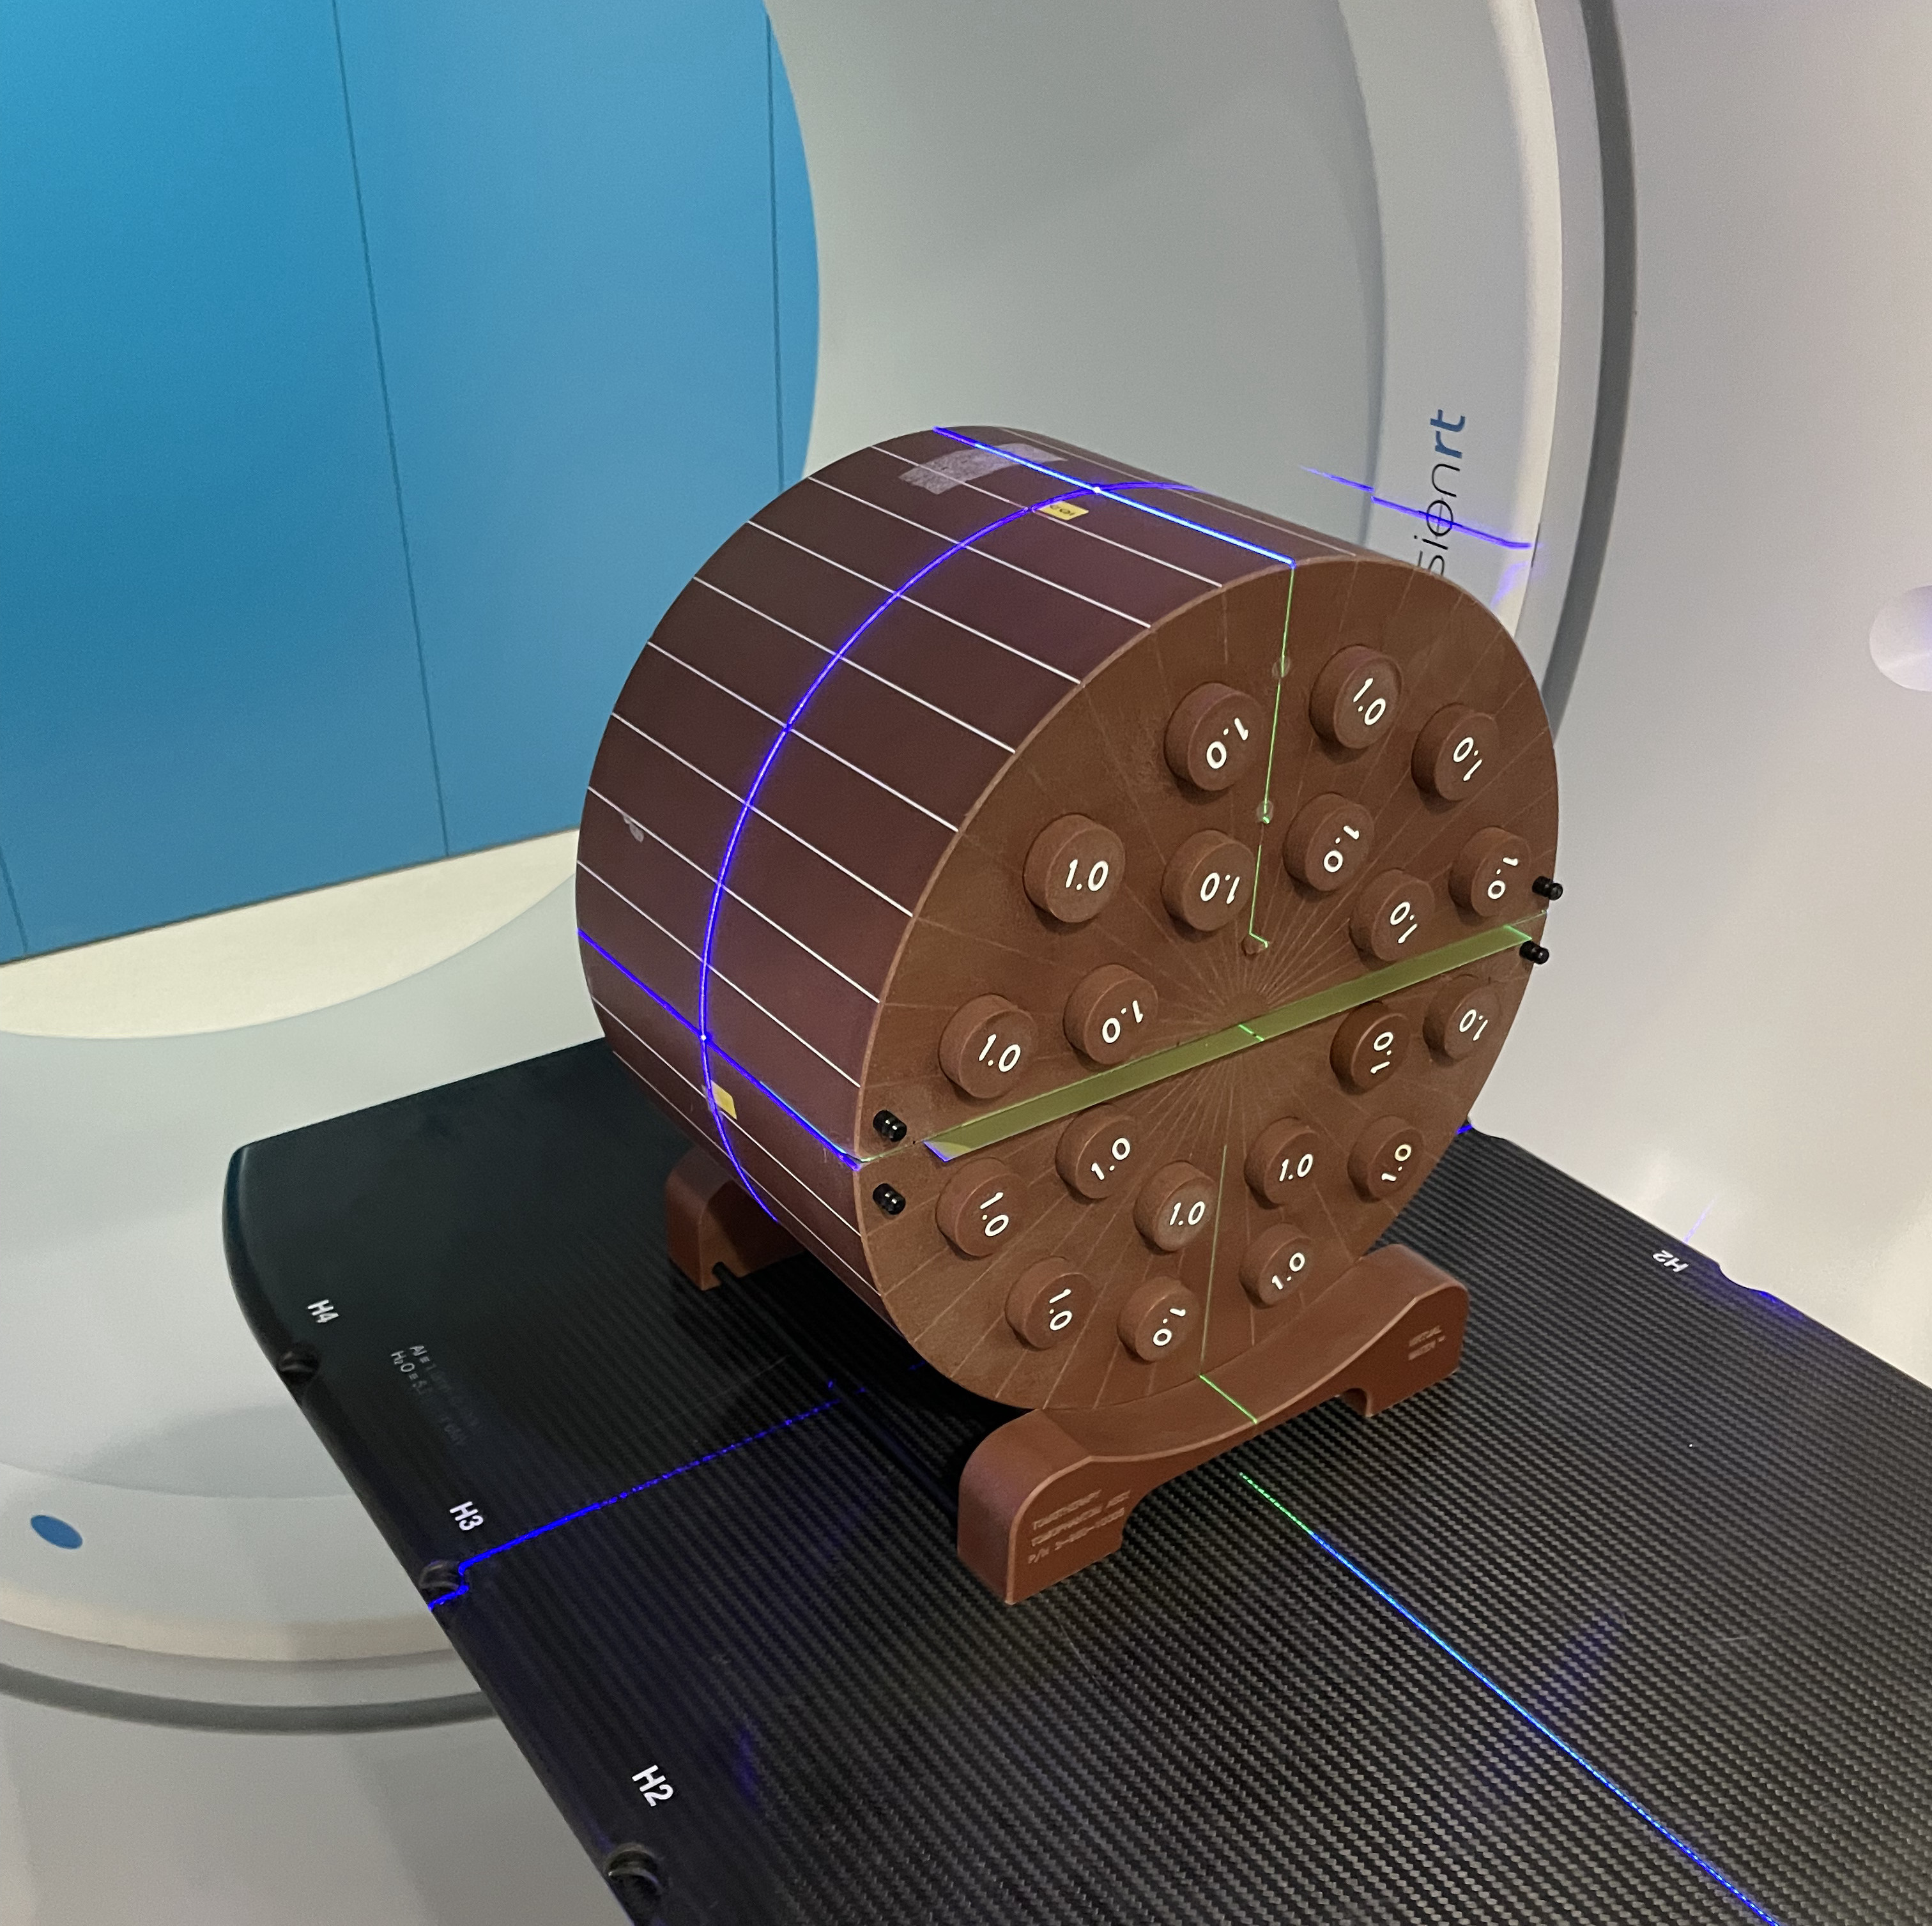
\includegraphics[scale=0.075]{figures/cheese.jpg}
  \caption{Placement du fantôme Cheese à l'Halcyon pour un contrôle patient à l'aide de films}
  \label{fig_DQP_films}
\end{figure}

Pour vérifier la distribution de dose acquise avec le film, nous avons calculé à l'aide de \textit{RayStation} cette distribution dans le fantôme Cheese, dans la même configuration que la mesure. La distribution calculée est ensuite exportée en RTPlan et RTDose au format DICOM. Le logiciel \textit{VeriSoft} est utilisé pour comparer la mesure avec le calcul en effectuant le calcul du gamma-index local, dont la définition est donnée en Annexe.

\subsection{Incertitudes}

Le rapport TG-235 de l'AAPM \cite{niroomand2020report} (\textit{The American Association of Physicists in Medicine}) indique plusieurs source d'incertitudes :

\begin{itemize}
  \item[$\bullet$] 0,9\% pour l'étalonnage des films
  \item[$\bullet$] 1,5\% concernant l'uniformité du film
  \item[$\bullet$] 1,5\% sur les paramètres d'ajustement utilisés lors de l'étalonnage
  \item[$\bullet$] 0,5\% sur les propriétés du scanner (3\% sur la valeur du pixel dans la zone homogène selon une étude interne antérieure)
  \item[$\bullet$] incertitude limitée pour l'uniformité du faisceau dû à une ROI de petite taille relativement à celle du faisceau
\end{itemize}

Pour calculer l'incertitude globale liée à la mesure de la dose avec des films, nous avons utilisé la formule suivante :

\begin{equation}
 \dfrac{u(y)}{y} = \sqrt{\sum\limits_i \left(\dfrac{u(x_i)}{x_i}\right)^2}
\end{equation}

Avec $\dfrac{u(y)}{y}$ l'incertitude globale et $\dfrac{u(x_i)}{x_i}$ l'incertitude liée aux différentes sources citées précédemment. Après calcul, nous obtenons une incertitude globale de 3,8\%.

\section{Matrices}

Les matrices de détecteurs ont servi dans ce travail à mesurer des profils de dose et des facteurs d'ouverture du collimateur (FOC). Dans cette optique, les caractéristiques des matrices sont présentées dans le tableau \ref*{table_matrices_caracteristiques} (les caractéristiques de toutes les matrices du centre sont fournies dans le tableau \ref*{fig_matrices_centre}).

\begin{table}[h]
  \centering
  \begin{tabular}{>{\centering\arraybackslash}m{1.3cm}>{\centering\arraybackslash}m{2cm}>{\centering\arraybackslash}m{2.2cm}>{\centering\arraybackslash}m{1.5cm}>{\centering\arraybackslash}m{1.5cm}>{\centering\arraybackslash}m{2cm}>{\centering\arraybackslash}m{3cm}}
    \toprule
    \textbf{Modèle} & \textbf{Constructeur} & \textbf{Champ maximal (cm}$\mathbf{^2}$\textbf{)} & \textbf{Nombre de chambres} & \textbf{Type de chambre}s & \textbf{Volume des chambres (cm}$\mathbf{^3}$\textbf{)} & \textbf{Commentaires} \\
    \toprule
    1500 & PTW & 27$\times$27 & 1405 & Chambres parallèles à air & 0,06 & Chambres en quinconce espacées de 1 cm \\ \hline
    1600 SRS & PTW & 15$\times$15 & 1521 & Chambres liquides & 0,003 & 2,5 mm entre les chambres (6,5$\times$6,5 cm$^2$) et 5 mm jusqu'à 15$\times$15 cm$^2$ \\
    \bottomrule
  \end{tabular}
  \caption{Caractéristiques des matrices utilisées}
  \label{table_matrices_caracteristiques}
\end{table}

\subsection{Étalonnage}

Pour chaque utilisation de la matrice, il est important d'élalonner le détecteur après l'avoir pré-irradiée d'une certaine quantité d'unités moniteur et avoir réalisé un zéro. Pour cela, la matrice est irradiée avec un champ et une dose connue. La dose mesurée par la chambre centrale permet d'appliquer un facteur correctif à l'ensemble des autres chambres de la matrice.

\subsection{Mesures de la dose}

Concernant les matrices, nous avons mesuré des profils et des FOC à l'aide du logiciel \textit{BeamAdjust} de PTW (version 2.3). Pour cela, nous avons utilisé 9,5 cm de plaques de RW3 au dessus (profondeur équivalent à 10 cm d'eau) et 5 cm en dessous de la matrice pour le rayonnement rétrodiffusé.

\subsubsection{Profils}

Les différents profils acquis à l'aide des matrices sont donnés dans le tableau \ref*{table_profils_matrices}. Ces mêmes mesures ont été effectuées pour les deux énergies disponibles pour les faisceaux de photons du Clinac 2, soit 6 MV et 23 MV. Les tailles de champ sont définies à l'aide des mâchoires.

\begin{table}[h]
  \centering
  \begin{tabular}{ccc}
  \toprule
  \textbf{Matrice} & \textbf{Champ} \textbf{(cm}$\mathbf{^2}$\textbf{)}\\ \toprule
  \multirow{2}{*}{1500} & 3$\times$3 \\
    & 10$\times$10 \\ \hline
  \multirow{2}{*}{1600 SRS} & 3$\times$3 \\
    & 10$\times$10 \\ \bottomrule
  \end{tabular}
  \caption{Profils de dose réalisés avec les matrices}
  \label{table_profils_matrices}
\end{table}

\subsubsection{FOC}

Les différents FOC acquis à l'aide des matrices sont donnés dans le tableau \ref*{table_foc_matrices}. Ces mêmes mesures ont été effectuées pour les deux énergies disponibles pour les faisceaux de photons du Clinac 2, soit 6 MV et 23 MV. Concernant les acquisitions des FOC avec les films EBT4, celles-ci n'ont pas pu être réalisées sur le même accélérateur puisque celui-ci est tombé en panne. Nous nous sommes donc servis d'un autre accélérateur disponible au centre, le Clinac iX100 du constructeur Varian qui peut délivrer des faisceaux de photons de 4 MV et de 10 MV.

% Des mesures de FOC ont également été faites avec des films EBT4. Cependant, l'accélérateur utilisé pour les autres détecteurs (Clinac 2) est tombé en panne. Le Clinac 3 a donc été utilisé avec l'énergie de 4 MV. La figures \ref*{fig_foc_films_C3_X4} et le tableau \ref*{table_foc_C3_X4} représente les résultats obtenus.

\begin{table}[h]
  \centering
  \begin{tabular}{cc}
  \toprule
  \textbf{Matrice} & \textbf{Champ (cm}$\mathbf{^2}$\textbf{)}\\ \toprule
  \multirow{7}{*}{1500 et 1600 SRS} & 3$\times$3 \\
   & 6$\times$6 \\
   & 8$\times$8 \\
   & 10$\times$10 \\
   & 12$\times$12 \\
   & 15$\times$15 \\ \bottomrule
  \end{tabular}
  \caption{FOC réalisés avec les matrices}
  \label{table_foc_matrices}
\end{table}

\subsection{Orientation de la matrice}

Des profils de dose à l'aide de la matrice 1500 du constructeur PTW ont été acquis au Clinac 3, avec un faisceau de 10 MV. Nous avons fait varier l'orientation de la matrice pour observer si cela impacte sur les différentes caractéristiques des profils de dose. Nous avons orienté la matrice suivant quatre angulations comme l'illusrte la figure \ref*{fig_orientations_matrice}.

\begin{figure}[h]
  \centering
  \includegraphics[scale=0.4]{figures/orientations_matrices.png}
  \caption{Schéma représentant les différentes orientation de la matrice 1500 lors des acquisitions de profils de dose au Clinac 3}
  \label{fig_orientations_matrice}
\end{figure}

\section{Détecteurs ponctuels}

Les chambres d'ionisation sont utilisées de manière récurrente en routine clinique pour le contrôle du débit de référence des accélérateurs ou encore pour des contrôles mensuels par exemple. Ils sont très pratiques puisqu'ils donnent une réponse instantanée et il est très simple de les installer. Le matériel utilisé pour ces mesures est mentionné dans le tableau \ref*{table_detecteurs_ponctuels}.

\begin{table}[h]
  \centering
  \begin{tabular}{ccccc}
    \toprule
    \textbf{Détecteur} & \textbf{Constructeur} &  \textbf{N}$\mathbf{^{\circ}}$ \textbf{de série} & \textbf{Volume (cm}$\mathbf{^3}$\textbf{)} & \textbf{Orientation du détecteur}\\
    \toprule
    Farmer & PTW & 011924 & 0,6 & Perpendiculaire \\
    CC13 & IBA & 3924 & 0,13 & Perpendiculaire \\
    MicroDiamant & PTW & 122271 & 0,004$\times$10$^{-3}$ & Parallèle \\
    Diode SRS & PTW & 000186 & 0,03 $\times$10$^{-3}$ & Parallèle \\
    Pinpoint & PTW & 00787 & 0,015 & Perpendiculaire \\
    \bottomrule
  \end{tabular}
  \caption{Détecteurs ponctuels utilisés}
  \label{table_detecteurs_ponctuels}
\end{table}

\subsection{Profils de dose}

Comme pour les rendements, les profils de dose ont été acquis avec la cuve à eau Blue Phantom 2. La DSP est également de 100 cm et les profils sont obtenus en faisant se déplacer le détecteur de manière perpendiculaire au faisceau à 10 cm de profondeur.

\subsection{Rendements en profondeur}

Pour acquérir des rendements en profondeur, nous avons utilisé la cuve à eau Blue Phantom 2 du constructeur IBA, ainsi que le logiciel associé MyQA. Cette cuve nous permet de déplacer dans les trois directions de l'espace le détecteur installé pour mesurer la distribution de dose du faisceau.

Les rendements s'obtiennent en faisant déplacer le détecteur le long de l'axe du faisceau en choisissant la vitesse de déplacement. La DSP choisie est de 100 cm.

\subsection{FOC}

Les FOC sont mesurés à l'aide de la cuve à eau IBA. Ils sont normalisés à la dose obtenue avec un champ de 10$\times$10 cm$^2$. La DSP est de 100 cm et une profondeur d'acquisition est de 10 cm.

%%%%%%%%%%%%%%%%%%%%%%%%%%%%%

\chapter{Résultats et discussions}
\section{Films}
\subsection{Courbe d'étalonnage}

La figure \ref*{fig_reponse_canaux} nous montre la réponse des trois canaux rouge, vert et bleu en fonction de la dose reçue par les films. Pour connaître la dose délivrée sur un film, une interpolation polynômiale de degré 3 a été effectuée sur les canaux rouge et vert comme le montre la figure \ref*{fig_courbe_etalonnage}\footnote{Le canal rouge est choisi pour les doses allant de 0 à 5 Gy, puis le canal vert est utilisé pour les doses allant de 5 à 10 Gy. Le canal bleu étant celui avec la plus forte pente sur toute la gamme de dose, il ne sera pas utilisé dans cette étude.}. Pour se rendre compte de la dépendance en énergie de la courbe d'étalonnage, nous avons réalisé une courbe pour chacune des énergies du Clinac 2 (6 MV et 23 MV), et nous avons effectivement constaté que la dépendance énergétique des films est très faible comme le montre la figure \ref*{fig_comp_canal_rouge} en Annexe (dans la gamme d'énergie utilisée en radiothérapie externe). Le tableau \ref*{table_ecart_dose_X6_X23}, en Annexe, nous montre les écarts de dose entre les deux courbes d'étalonnage. Les écarts sont importants pour les faibles doses (21,87\% d'écart entre la dose mesurée avec la chambre d'ionisation et celle calculée à l'aide de la courbe d'étalonnage en 23 MV pour 0,1 Gy délivré).


\begin{figure}[h]
  \centering
  \includegraphics[scale=0.4]{figures/reponse_trois_canaux.PNG}
  \caption{Valeur de pixel en fonction de la dose pour les trois canaux rouge vert et bleu acquis à l'aide du scanner Epson Expression 1200 XL (faisceau de 6 MV)}
  \label{fig_reponse_canaux}
\end{figure}

\begin{figure}[h]
  \centering
  \includegraphics[scale=0.5]{figures/etalonnage_X6.PNG}
  \caption{Courbe d'étalonnage des films pour un faisceau de 6 MV}
  \label{fig_courbe_etalonnage}
\end{figure}

\newpage
\subsection{Rendements en profondeur}

Les rendements en profondeur ont été acquis avec une très bonne résolution spatiale grâce aux fims radiochromiques (0,338 mm en prenant en compte la taille du pixel) mais avec un bruit important (malgré un filtre médian), comme le montre la figure \ref*{fig_rdt_films_X6_X23}. De plus, nous voyons que l'orientation du film dans le scanner impacte de manière non négligeable la quantification de dose absorbée sur le film\footnote{Rappelons que la courbe d'étalonnage a été établie en scannant les films en mode portait}. Il faut également prendre en compte la zone homogène du scanner puisque celle-ci est restreinte et est plus petite que celle du film si celui-ci est orienté en mode paysage. 

\begin{figure}[h]
  \centering
  \includegraphics[scale=0.5]{figures/rdt_X6_X23_portrait_paysage.PNG}
  \caption{Rendements en profondeur acquis à l'aide de films pour les faisceaux de 6 MV et de 23 MV (DSP = 100 cm). Scan réalisé en portait et en paysage}
  \label{fig_rdt_films_X6_X23}
\end{figure}

Pour voir l'influence de l'orientation du film lors de la numérisation, nous pouvons représenter les PV en fonction de la profondeur sur la figure \ref*{fig_fading_PV}. Nous voyons que pour les deux énergies de l'accélérateur, le mode paysage donne une réponse plus importante en valeur de pixel (ce qui sous estime la dose), il est donc très important de garder la même orientation des films dans le scanner qu'à l'étalonnage. Nous n'observons pas autant de différence sur la figure \ref*{fig_rdt_films_X6_X23} car la dose mesurée pour toutes les profondeurs a été normalisée.

\newpage
\begin{figure}[h]
  \centering
  \includegraphics[scale=0.5]{figures/rdt_PV_portrait_paysage.PNG}
  \caption{PV en fonction de la profondeur, orientation du film en portrait et en payage pour les des faisceaux de 6 MV et de 23 MV. DSP de 100 cm et champ 10$\times$10 cm$^2$ à la surface}
  \label{fig_fading_PV}
\end{figure}

\subsection{FOC}

Les résultats des FOC sont donnés sur la figure \ref*{fig_foc_films}. Les FOC se calculant grâce à un rapport entre deux doses mesurées où l'incertitude associée est de 3,8\% pour chacune, nous avons donc utilisé une somme quadratique pour calculer l'incertitude sur les FOC, soit une incertitude de 5,3\% sur chacun des points.

Nous voyons que les valeurs de FOC du commissionning sont à l'interieur des barres d'erreurs associées aux FOC des films mais qui sont tout de même très étendues. La tendance reste la même pour les deux mesures.

\begin{figure}[h]
  \centering
  \includegraphics[scale=0.6]{figures/foc_incertitudes_X4.PNG}
  \caption{FOC acquis avec des films radiochromiques. DSD de 100 cm.}
  \label{fig_foc_films}
\end{figure}

\begin{table}[h]
  \centering
  \begin{tabular}{cccc}
  \hline
  \textbf{Champ carré (cm)} & \textbf{FOC film} & \textbf{FOC commissionning} & \textbf{Ecart relatif (\%)}\\ \hline
  2 & 0,76 & 0,77 & 0,76 \\
  3 & 0,82 & 0.808 & 2,03 \\
  6 & 0,91 & / & / \\
  8 & 0,96 & / & / \\
  10 & 1,00 & 1,00 & 0 \\
  12 & 1,02 & / & / \\
  15 & 1,05 & 1,075 & 2,64 \\
  20 & 1,06 & 1,13 & 6,28 \\ \hline
  \end{tabular}
  \caption{FOC obtenus à l'aide de films EBT4. DSP de 90 cm, DSD de 100 cm et énergie de 4 MV (Clinac 3)}
  \label{table_foc_C3_X4}
\end{table}

\newpage
\subsection{Étude de la réponse en fonction du délai de lecture après irradiation}

La figure \ref*{fig_fading} nous montre l'évolution de la PV (et donc de la dose) en fonction du temps entre l'iradiation et la numérisation. Nous voyons que jusqu'à 10 heures après irradiation, la quantification de la dose sur le film est sous-estimée (la dose réelle est de 2 Gy, ce qui correspond à 254 UM pour un faisceau de 6 MV au Clinac 2). N ous pouvons conclure qu'après un délai de 10h, le phénomène de polymérisation se stabilise.

\begin{figure}[h]
  \centering
  \begin{minipage}{.47\linewidth}
    \includegraphics[scale=0.6]{figures/fading_PV.PNG}
  \end{minipage}
  \begin{minipage}{.47\linewidth}
    \includegraphics[scale=0.6]{figures/fading_dose.PNG}
  \end{minipage}
  \caption{Étude de la réponse en fonction du délai de lecture après irradiation (en PV à gauche et en dose à droite)}
  \label{fig_fading}
\end{figure}

\subsection{Plan de traitement}

La comparaison entre la distribution de dose calculée sur \textit{RayStation} et la mesure avec les films est observable sur la figure \ref*{fig_dose_map_VS} et le tableau \ref*{table_gamma_index}. Il en est de même pour la matrice 1500 sur la figure \ref*{fig_dose_map_matrice}.

\begin{figure}[h]
  \centering
  \includegraphics[scale=0.4]{../captures/VS_3_3.PNG}
  \caption{Comparaison des plans calculé et mesuré sur le logiciel \textit{VeriSoft} (3\% 3mm)}
  \label{fig_dose_map_VS}
\end{figure}

\begin{figure}[h]
  \centering
  \includegraphics[scale=0.7]{figures/DQA_matrice_comp.png}
  \caption{Comparaison des plans calculé et mesuré avec la matrice 1500 sur le logiciel \textit{VeriSoft} (3\% 3 mm)}
  \label{fig_dose_map_matrice}
\end{figure}

\begin{table}[h]
  \centering
  \begin{tabular}{|ccc|cc|}
  \hline
  \multicolumn{3}{|c|}{\textbf{Matrice}}                                 & \multicolumn{2}{c|}{\textbf{Film}}                       \\ \hline
  \multicolumn{3}{|c|}{\textbf{3\%/3mm}}                                 & \multicolumn{1}{c|}{\textbf{3\%/3mm}} & \textbf{5\%/3mm} \\ \hline
  \multicolumn{1}{|c|}{\textbf{10\%}} & \multicolumn{1}{c|}{\textbf{70\%}} & \textbf{90\%} & \multicolumn{1}{c|}{\multirow{2}{*}{87,60\%}} & \multirow{2}{*}{95,10\%} \\ \cline{1-3}
  \multicolumn{1}{|c|}{92,70\%} & \multicolumn{1}{c|}{97,80\%} & 93,40\% & \multicolumn{1}{c|}{}                 &                  \\ \hline
  \end{tabular}
  \caption{Résultats du gamma index local (3D pour la matrice et 2D pour les films) donnés par \textit{VeriSoft} pour l'analyse des plans de traitement}
  \label{table_gamma_index}
  \end{table}

Nous pouvons voir qu'il y a des différences notables entre le calcul de la distribution de dose et la mesure du plan de traitement du patient avec le film. Cela peut s'expliquer par le fait que le film est bien plus grand que la zone homogène du scanner mais aussi, comme nous l'avons déjà vu précédemment, le signal du film après numérisation est plutôt bruité.

La figure \ref*{fig_profil_h_v_VS} montre la comparaison de profils de dose entre les deux distributions (calculée et mesurée). Nous voyons que le film permet une très bonne restitution des gradients de dose grâce à sa bonne résolution spatiale. Cependant, nous pouvons noter qu'il y a des différences en terme de quantification de dose puisque la dose mesurée sur le film n'est pas toujours semblable à la dose calculée par le TPS (points rouges et bleus sur les figures \ref*{fig_dose_map_VS} et \ref*{fig_profil_h_v_VS} qui correspondent à un surdosage et un sous-dosage respectivement).

\begin{figure}[h]
  \centering
  \begin{minipage}{.45\linewidth}
    \includegraphics[scale=0.4]{figures/profil_h_VS.png}
  \end{minipage}
  \begin{minipage}{.45\linewidth}
    \includegraphics[scale=0.4]{figures/profil_v_VS.png}
  \end{minipage}
  \caption{Profils de dose en horizontal (à gauche) et vertical (à droite) pour la mesure avec le film et le calcul}
  \label{fig_profil_h_v_VS}
\end{figure}

La figure \ref*{fig_histo} nous montrent les histogrammes du gamma index local pour les critères 3\% 3 mm et 5\% 3 mm. Nous pouvons voir que la majorité des points examinés qui ne répondent pas aux critères sont des points de faibles doses. Il serait peut-être intéressant d'établir une courbe d'étalonnage avec plus de points dans les faibles doses pour minimiser les incertitudes de mesure.

\begin{figure}[h]
  \centering
  \begin{minipage}{.4\linewidth}
    \includegraphics[scale=0.5]{../captures/VS_histogramme_3_3.PNG}
  \end{minipage}
  \begin{minipage}{.4\linewidth}
    \includegraphics[scale=0.5]{../captures/VS_histogramme_5_3.PNG}
  \end{minipage}
  \caption{Histogrammes du gamma index pour les critères 3\% 3 mm (à gauche) et 5\% 3mm (à droite)}
  \label{fig_histo}
\end{figure}

% \begin{figure}[h]
%   \centering
  
%   \caption{Histogramme du gamma index pour le critère 3\% 3mm}
%   \label{fig_histo_3_3}
% \end{figure}

% \begin{figure}[h]
%   \centering
  
%   \caption{Histogramme du gamma index pour le critère 5\% 3mm}
%   \label{fig_histo_5_3}
% \end{figure}

\subsection{Orientation de la matrice}

Les résultats sont présentés sur la figure \ref*{fig_resultats_profils_matrice} et le tableau \ref*{table_resultats_profils_matrice}. Nous pouvons voir que l'orientation de la matrice n'influence quasiment pas les résultats. En effet, nous voyons que la pénombre est très sensiblement la même, surtout lorsque les orientations sont opposées. Il en est de même pour l'homogénéité et la symétrie. Notons que la matrice est utilisée à 180$^{\circ}$ lors des contrôles des plans des patients en routine clinique.

\begin{figure}[h]
  \centering
  \includegraphics[scale=0.4]{figures/CQ_matrice_1500.png}
  \caption{Profils de dose acquis avec la matrice PTW 1500 pour différentes orientations. DSD de 100 cm et DSP 90,5 cm.}
  \label{fig_resultats_profils_matrice}
\end{figure}

\begin{table}[h]
  \centering
  \begin{tabular}{ccccc}
  \toprule
  \textbf{Orientation ($\mathbf{^{\circ}}$\textbf{)}} & \textbf{H (\%)} & \textbf{S (\%)} & \textbf{Pénombre G (mm)} & \textbf{Pénombre D (mm)} \\ \toprule
  0 & 2,00 & 0,81 & 15,03 & 14,96 \\
  90 & 2,04 & 0,56 & 15,26 & 15,21 \\
  180 & 1,97 & 0,72 & 15,03 & 15,01 \\
  270 & 2,06 & 0,53 & 15,30 & 15,09 \\ \bottomrule
  \end{tabular}
  \caption{Résultats fournis par le logiciel \textit{BeamAdjust} pour les différents profils (Faisceau de 10 MV au Clinac 3)}
  \label{table_resultats_profils_matrice}
\end{table}

\section{Comparaison des détecteurs}
\subsection{Profils de dose}

Les figures \ref*{fig_profils_3x3}  et \ref*{fig_profils_10x10} ainsi que le tableau \ref*{table_resultats_detecteurs_FOC} nous donnent les résultats des profils de dose pour tous les détecteurs utilisés lors des manipulations pour des champs de 3$\times$3 cm$^2$  et 10$\times$10 cm$^2$ respectivement. Les tailles de champ acquises avec les films et la matrice 1500 sont plus petites que pour les autres détecteurs. En effet, pour les acquisitions avec les détecteurs ponctuels, la cuve Blue Phantom 2 du constructeur IBA a été utilisée à une DSP de 100 cm et une profondeur de 10 cm alors que pour les films et les matrices, la distance source-détecteur est de 100 cm (utilisation de mesures réalisées précédemment).

\begin{figure}[h]
  \centering
  \includegraphics[scale=0.35]{figures/3x3_comp.PNG}
  \caption{Profils de dose 3$\times$3 cm$^2$ pour différents détecteurs. Orientation \textit{crossline}.}
  \label{fig_profils_3x3}
\end{figure}

Les films nous permettent d'avoir une pénombre plus réduite (gradient de dose plus important) puisque leur résolution spatiale est bien meilleure que les autres détecteurs, mais possèdent un signal assez bruité. Concernant les matrices, nous voyons que la PTW 1500 est très peu résolue, ce qui engendre une pénosmbre plus importante (voir tableau \ref*{table_profils_matrices}). La matrice 1600 quant à elle permet d'obtenir plus de points sur la courbe de profils de dose grâce à une meilleure résolution que la matrice 1500 (voir les caractéristiques des matrices dans les tableaux \ref*{table_matrices_caracteristiques} et \ref*{fig_matrices_centre}). À propos des détecteurs ponctuels, nous voyons sur tableau \ref*{table_resultats_detecteurs_FOC} que la pénombre pour l'ensemble des détecteurs ponctuels est plus faible. L'utilisation de la cuve à eau permet de mesurer des gradients de dose plus importants puisqu'elle proposent des vitesses d'intégration basses.

% \begin{table}[h!]
%   \centering
%   \begin{tabular}{>{\centering\arraybackslash}m{1.7cm}>{\centering\arraybackslash}m{2cm}>{\centering\arraybackslash}m{2cm}>{\centering\arraybackslash}m{2.5cm}>{\centering\arraybackslash}m{2.2cm}>{\centering\arraybackslash}m{3cm}}
%     \toprule
%     \textbf{Détecteur} & \textbf{Symétrie (\%)} & \textbf{Homogénéité (\%)} & \textbf{Centre du champ (cm)} & \textbf{Pénombre G-D (cm)} & \textbf{Taille de champ (cm)} \\
%     \toprule
%     CC13 & 100,56 & 2,25 & -0,05 & 0,68 - 0,68 & 11,07 \\
%     Diode & 101,01 & 2,64 & -0,02 & 0,45 - 0,44 & 11,11 \\
%     MicroDiamant & 101,72 & 2,91 & -0,04 & 0,38 - 0,4 & 11,04 \\
%     Pinpoint & 101,99 & 2,68 & -0,02 & 0,65 - 0,65 & 11,07 \\
%     \bottomrule
%   \end{tabular}
%   \caption{Influence du détecteur sur les profils pour un champ 10$\times$10 cm$^2$ (résultats MyQA)}
%   \label{table_profils_detecteurs_ponctuels}
% \end{table}

\begin{figure}[h]
  \centering
  \includegraphics[scale=0.4]{figures/10x10_comp.PNG}
  \caption{Profils de dose 10$\times$10 cm$^2$ pour différents détecteurs. Orientation \textit{crossline}.}
  \label{fig_profils_10x10}
\end{figure}

\begin{table}[h]
  \centering
  \begin{tabular}{>{\centering\arraybackslash}m{1.5cm}>{\centering\arraybackslash}m{2.3cm}>{\centering\arraybackslash}m{2cm}>{\centering\arraybackslash}m{2cm}>{\centering\arraybackslash}m{2cm}>{\centering\arraybackslash}m{2cm}>{\centering\arraybackslash}m{1.5cm}}
  \toprule
  \textbf{Champ (cm}$\mathbf{^2}$\textbf{)} & \textbf{Détecteur} & \textbf{Homogénéité (\%)} & \textbf{Symétrie (\%)} & \textbf{Pénombre gauche (mm)} & \textbf{Pénombre droite (mm)} & \textbf{DSP (cm)}\\ \toprule
  \multirow{7}{*}{10$\times$10} & Matrice 1500 & 4,66 & 2,57 & 14,12 & 14,34 & 90 \\
   & Matrice 1600 & 2,2 & 1,25 & 7,43 & 7,16 & 90 \\
   & CC13 & 2,55 & 100,56 & 0,68 & 0,68 & 100 \\
   & Diode & 2,64 & 101,01 & 0,45 & 0,45 & 100 \\
   & MicroDiamant & 2,91 & 101,72 & 0,38 & 0,34 & 100 \\
   & Pinpoint & 2,68 & 101,99 & 0,65 & 0,65 & 100 \\
   & Films & / & / & 0,37 & 0,35 & 90\\ \hline
  \multirow{7}{*}{3$\times$3} & Matrice 1500 & 1,05 & 100,81 & 3,74 & 3,62  & 90 \\ 
   & Matrice 1600 & 3,45 & 100,51 & 0,37 & 0,37  & 90 \\ 
   & CC13 & 7,9 & 100,28 & 0,56 & 0,55 & 100 \\
   & Diode & 3,23 & 100,68 & 0,30 & 0,31 & 100 \\
   & MicroDiamant & 3,98 & 101,33 & 0,31 & 0,30 & 100 \\
   & Pinpoint & 5,19 & 100,99 & 0,43 & 0,44 & 100 \\
   & Films & / & / & 0,23 & 0,27 & 90 \\
  \bottomrule
  \end{tabular}
  \caption{Résultats des logiciels \textit{BeamAdjust} et \textit{MyQA} pour les profils de dose pour l'ensemble des détecteurs utilisés dans ce rapport pour les champs 3$\times$3 cm$^2$ et 10$\times$10 cm$^2$}
  \label{table_resultats_detecteurs_FOC}
\end{table}

\subsection{Rendements en profondeur}

Les résultats des rendements en profondeur sont donnés dans le tableau \ref*{table_rdt_detecteurs_ponctuels}. Nous observons que le $z_{max}$ (ou $R_{100}$ dans le tableau) pour les films est plus faible que pour les autres détecteurs (sauf pour la diode). Les acquisitions des films étant très bruitées, il est difficile d'extraire la position du maximum de dose. Pour la diode, le volume sensible n'étant pas équivalent eau ($Z_{eff}$=14), la diode favorise l'effet photoélectrique : l'équilibre électronique est donc atteint plus rapidement. En ce qui concerne le placement des films entre les plaques, celui-ci est très peu reproductible puisqu'il est effectué manuellement, ce qui augmente les incertitudes sur la mesures de la dose avec ce type de détecteur.

\begin{table}[h]
  \centering
  \begin{tabular}{cccc}
    \toprule
    \textbf{Détecteur} & $\mathbf{R_{100}}$ \textbf{(cm)} & $\mathbf{R_{50}}$ \textbf{(cm)} & $\mathbf{D_{20}/D_{10}}$ \\
    \toprule
    CC13 & 1,35 & 14,98 & 0,571 \\
    Diode & 0,70 & 14,55 & 0,571 \\
    MicroDiamant & 1,57 & 14,72 & 0,572 \\
    Pinpoint & 1,46 & 15,65 & 0,593 \\
    Films & 1,19 & 12,46 & 0,565 \\
    \bottomrule
  \end{tabular}
  \caption{Résultats de l'influence du détecteur sur les rendements en profondeur pour le faisceau de photons de 6 MV du Clinac 2}
  \label{table_rdt_detecteurs_ponctuels}
\end{table}


Le tableau \ref*{table_epaisseurs_detecteurs} nous donne les épaisseurs de chacun des détecteurs utilisés pour les acquisitions de profils. L'épaisseur du détecteur utilisé a un impact sur le profil de dose puisque la réponse du détecteur est un signal moyen le long de cette épaisseur. Les films possédant une épaisseur active de 28 $\mu$m, comme le montre la figure \ref*{fig_couches_EBT4}, l'acquisition des rendements est très précise en profondeur comparé à la chambre CC13 par exemple qui est épaisse de 6 mm. Il en est de même pour le MicroDiamant qui est encore plus fin.

\begin{table}[h]
  \centering
  \begin{tabular}{cc}
    \toprule
    \textbf{Détecteur} & \textbf{Épaisseur (mm)} \\
    \toprule
    CC13 & 6 \\
    MicroDiamant & 1$\times$10$^{-3}$  \\
    Pinpoint & 0,3  \\
    Diode & 1  \\
    Matrice 1500 & 3 \\
    Matrice 1600 & 2,5 \\
    Films & 28$\times$10$^{-3}$ \\
    \bottomrule
  \end{tabular}
  \caption{Épaisseur de chacun des détecteurs utilisés}
  \label{table_epaisseurs_detecteurs}
\end{table}

\subsubsection{FOC}

Comme le montre la figure \ref*{fig_comp_foc_X6}, les différences entre les détecteurs se fait peu ressentir, sauf pour le champ de 3$\times$3 cm$^2$. En effet, la taille du volume sensible plus importante de la chambre Farmer par rapport à la chambre CC13 joue un rôle dans la quantification des charges collectées (0,6 cm$^3$ contre 0,13 cm$^3$ pour la CC13).

\begin{figure}[h]
  \centering
  \includegraphics[scale=0.39]{../scripts/figures/comp_foc_C2.png}
  \caption{FOC pour différents détecteurs. DSP de 90 cm, DSD de 100 cm et énergie de 6 MV (Clinac 2)}
  \label{fig_comp_foc_X6}
\end{figure}

De plus, la matrice 1600 SRS possède des chambres d'ionisation liquides, cela se manifeste par un signal reccueilli plus important que pour les autres détecteurs.

\chapter{Conclusion}

Pour conclure, nous avons pu voir durant ce travail que chacun des détecteurs utilisés ont leur lot d'avantages et d'invonvenients. Pour des contrôles de qualité en routine clinique, il est plus pratique d'utiliser des détecteurs ponctuels qui donnent une réponse immédiate avec un bon compromis entre résultat et temps d'installation (que ce soit pour les rendements en profondeur, les profils de dose ou les FOC) par rapport aux films et aux matrices.

Concernant le contrôle des plan de traitement des patients, l'utilisation de films radiochromiques est plus compliqué puisque le résultat n'est pas instantanné (réaction de polymérisation) et dépend de beaucoup d'éléments de la chaine de mesure (placement du film avant irradiation, incertitudes liées au scanner, traitement d'image...). L'utilisation d'une matrice associée à un fantôme adapté est certes moins résolue mais donne de meilleurs résultats et reste plus pratique à utilisé en routine clinique. Les films radiochromiques peuvent être utiles pour la validation d'un modèle de faisceau et pour la mise en service d'un accélérateur avant le traitement des patients.

\chapter{Annexe}

\begin{figure}[h]
  \centering
  \includegraphics[scale=0.6]{figures/reponse_X23.PNG}
  \caption{Valeur de pixel en fonction de la dose pour les trois cannaux rouge, vert et bleu acquis à l'aide du scanner Epson Expression 12000 XL (faisceau de 23 MV)}
  \label{fig_reponse_scanner_X23}
\end{figure}

\begin{figure}[h]
  \centering
  \includegraphics[scale=0.6]{figures/etalonnage_X23.PNG}
  \caption{Courbe d'étalonnage des films pour un faisceau de 23 MV}
  \label{fig_courbe_etalonnage_X23}
\end{figure}

\begin{figure}[h]
  \centering
  \includegraphics[scale=0.4]{figures/comp_X6_X23_canal_rouge.PNG}
  \caption{Comparaison de la dose en fonction de la valeur de pixel pour le canal rouge du scanner avec un faisceau de 6 MV et un faisceau de 23 MV}
  \label{fig_comp_canal_rouge}
\end{figure}

\begin{table}[h]
  \begin{tabular}{>{\centering\arraybackslash}m{2cm}>{\centering\arraybackslash}m{2cm}>{\centering\arraybackslash}m{2cm}>{\centering\arraybackslash}m{2cm}>{\centering\arraybackslash}m{2cm}>{\centering\arraybackslash}m{2cm}>{\centering\arraybackslash}m{2cm}}
  \toprule
  \textbf{Dose   réelle (Gy)} &
    \textbf{Dose calculée X6 (Gy)} &
    \textbf{Dose calculée X23   (Gy)} &
    \textbf{Dose calculée X4 (Gy)} &
    \textbf{Ecart relatif X6} &
    \textbf{Ecart relatif X23} &
    \textbf{Ecart relatif X4} \\ \toprule
  0,10 & 0,086 & 0,078 & 0,108 & -14,09\% & -21,87\% & 7,75\%  \\
  0,30 & 0,320 & 0,319 & 0,315 & 6,44\%   & 6,42\%   & 5,03\%  \\
  0,50 & 0,481 & 0,502 & 0,501 & -3,79\%  & 0,23\%   & 0,10\%  \\
  0,70 & 0,721 & 0,709 & 0,726 & 3,01\%   & 1,29\%   & 3,76\%  \\
  1,00 & 0,970 & 0,992 & 1,002 & -2,99\%  & -0,74\%  & 0,19\%  \\
  1,50 & 1,534 & 1,507 & 1,465 & 2,29\%   & 0,46\%   & -2,35\% \\
  2,00 & 1,961 & 1,978 & 1,989 & -1,92\%  & -1,06\%  & -0,51\% \\
  3,00 & 3,047 & 3,021 & 2,969 & 1,56\%   & 0,68\%   & -1,03\% \\
  4,00 & 3,957 & 3,999 & 4,102 & -1,07\%  & -0,03\%  & 2,54\%  \\
  5,00 & 5,010 & 4,997 & 4,941 & 0,20\%   & -0,05\%  & -1,19\% \\ \bottomrule
  \end{tabular}
  \caption{Comparaison de la dose déposée sur les films pour les faisceaux de 4 MV, 6 MV, 23 MV}
  \label{table_ecart_dose_X6_X23}
\end{table}

\newpage
\paragraph*{Définition du gamma-index :}

Le gamma-index permet d'évaluer quantitativement la concordance de deux distributions de dose (voir figure \ref*{fig_gamma_index}). Le gamma-index est considéré comme validé si sa valeur est inférieure à 1 pour chacun des points de la distribution de dose. Pour cela, il faut respecter le critère en dose ($DD_{max}$) et le critère en distance ($DTA$). Le score du gamma-index représente le pourcentage de points de la distribution de dose pour lesquels le gamma-index est inférieur ou égal à 1.

\begin{figure}[h]
  \centering
  \includegraphics[scale=0.4]{figures/schema_gamma_index.png}
  \caption{Évaluation de la concordance entre deux distributions de dose à l'aide du gamma-index (le gamma-index est représenté par les ellipsoïdes)}
  \label{fig_gamma_index}
\end{figure}

Il existe deux types de gamma-index. Le gamma-index global et le gamma-index local dont les définitions sont données comme suit :

\begin{itemize}
  \item[$\bullet$] gamma-index global : le DDmax est constant pour tous les points de la distribution de dose. Valeur prise sur un point de référence (centre de la matrice de référence, valeur maximale, centre de gravité, ...)
  \item[$\bullet$] gamma-index local : le DDmax varie pour chaque point, le pourcentage s’applique au point d’intérêt. Plus sensible pour les zones de faibles doses
\end{itemize}

\newpage

\begin{figure}[h]
  \centering
  \includegraphics[scale=0.5]{figures/couches_film_EBT4.png}
  \caption{Structure des films Gafchromic$^{\text{TM}}$ EBT4 \cite{EBT4brochure}}
  \label{fig_couches_EBT4}
\end{figure}

\begin{figure}[h]
  \centering
  \includegraphics[scale=0.55]{figures/courbe_etalonnage_C3_X4.PNG}
  \caption{Courbe d'étalonnage des films EBT4 réalisée sur le Clinac 3 en X4}
  \label{fig_courbe_etalonnage_X4}
\end{figure}

\begin{figure}[h]
  \centering
  \includegraphics[scale=0.5]{figures/tableau matrices.PNG}
  \caption{Caractéristiques des matrices utilisées sur site}
  \label{fig_matrices_centre}
\end{figure}

\clearpage
\bibliography{biblio}
\bibliographystyle{plain}
\nocite{*}

\end{document}